\chapter{Phương án đề xuất}
\label{chap:phuong_an_de_xuat}
	\textit{Trong chương này, chúng tôi mô tả chi tiết bài toán trước khi bắt tay vào hiện thực.\linebreak Sau đó, chúng tôi đề xuất kiến trúc mạng và các hàm lỗi sẽ sử dụng. Cuối cùng, chúng tôi đề xuất phương pháp tìm đường chính giữa và điểm phân nhánh của mạch máu.}
\minitoc

\section{Nội dung bài toán} 
\label{sec:noi_dung_bai_toan}
	Sau quá trình tìm hiểu và tổng hợp các kiến thức trong lĩnh vực Xử lý hình ảnh nói chung và Phân đoạn hình ảnh y khoa nói riêng, chúng tôi đưa ra bài toán để giải quyết đó là \textit{Phát hiện và xây dựng hệ thống mạch máu của gan từ ảnh chụp cắt lớp vi tính.}
	
	Hệ thống nhằm mục đích trực quan hoá hệ thống mạch máu bên trong cơ quan gan. Đồng thời thể hiện đường chính giữa mạch máu và các điểm phân nhánh, giúp xác định vị trí tương quan giữa các phân thuỳ gan, hỗ trợ công tác giải phẫu được tiến hành nhanh chóng và an toàn hơn.
	
	\textbf{Thông tin đầu vào (Input):} dữ liệu đầu vào của bài toán gồm hai phần: phần thứ nhất là các lớp ảnh CT cơ quan gan của một bệnh nhân bất kỳ, phần thứ hai là nhãn phân đoạn cơ quan gan tương ứng cho bộ ảnh CT đó.
	
	\textbf{Kết quả đầu ra (Output):} kết quả đầu ra của bài toán này bao gồm ba phần: phần thứ nhất là kết quả phân đoạn hệ thống mạch máu trong cơ quan gan từ khối ảnh CT, phần thứ hai là đường chính giữa của các mạch máu trong hệ thống mạch máu có được từ kết quả phân đoạn, phần cuối cùng là các điểm phân nhánh của mạch máu.
	
	Sau khi xác định thông tin đầu vào và kết quả đầu ra của bài toán, chúng tôi đề xuất phương án thiết kế hệ thống với những tham khảo từ các công trình liên quan được trình bày trong phần tiếp theo.

\section{Kiến trúc mạng và hàm lỗi} 
\label{sec:kien_truc_mang_va_ham_loi}
	Trong mục này, chúng tôi trình bày những kiến trúc mạng sẽ được sử dụng trong quá trình thí nghiệm và đánh giá. Những kiến trúc này bao gồm các kiến trúc được đề xuất trong các công trình liên quan và những cải tiến do chúng tôi đề xuất. Cuối cùng, chúng tôi đề xuất những hàm lỗi sẽ được sử dụng trong quá trình huấn luyện.
	
\subsection{Kiến trúc mạng} 
\label{subsec:kien_truc_mạng}
	Kiến trúc mạng chúng tôi sử dụng để thí nghiệm và đánh giá hệ thống trong đề tài này bao gồm mô hình DeepVesselNet và mô hình U-Net*.
	
	\textbf{DeepVesselNet}: đối với mô hình DeepVesselNet, chúng tôi hiện thực lại kiến trúc đã được đề xuất trong \cite{tetteh2018deepvesselnet}. Ngoài ra, chúng tôi đề xuất bổ sung lớp batchnorm\index{Batchnorm} trước các lớp ReLU trong kiến trúc này để đánh giá, so sánh.
	
	\textbf{U-Net*}: kiến trúc này được chúng tôi hiện thực dựa trên ý tưởng của mô hình U-Net đã được giới thiệu trong bài báo \cite{ronneberger2015u} cùng với những thay đổi cần thiết. Thay đổi đầu tiên được chúng tôi thực hiện là sử dụng các lớp convolution 3D thay cho các lớp convolution 2D. Lý do cho sự thay đổi này đến từ tính chất của tập dữ liệu. Khác với tập dữ liệu được sử dụng trong bài báo là những hình ảnh rời rạc về tế bào, trong đề tài này, chúng tôi sử dụng ảnh CT làm dữ liệu đầu vào với mỗi bộ ảnh là tập các hình ảnh thu được từ các lớp cắt liên tiếp nhau trên một phần cơ thể. Những lớp cắt này có mối liên hệ với nhau về mặt không gian. Ví dụ, tại một điểm trên một lớp cắt xuất hiện mạch máu thì xác suất xuất hiện mạch máu ở những vị trí lân cận trên các lớp liền kề là rất cao. Chúng tôi sử dụng lớp convolution 3D nhằm giúp mô hình có thể khai thác tốt hơn những đặc trưng từ dữ liệu dạng này. 
	
	Thay đổi tiếp theo được chúng tôi thực hiện trong quá trình hiện thực mô hình U-Net* liên quan đến độ sâu của kiến trúc mạng. Nhận thấy rằng kích thước đối tượng cần phân đoạn là mạch máu nhỏ hơn rất nhiều so với kích thước tế bào trong dữ liệu của bài báo và càng xuống sâu trong mô hình U-Net, kích thước dữ liệu càng bị thu giảm. Để những đặc trưng của mạch máu không bị mất đi cần thiết phải có sự điều chỉnh phù hợp trong độ sâu của mô hình. Chúng tôi tiến hành xác định kích thước mạch máu cần phân đoạn và tính toán receptive field cho mỗi lớp mạng của mô hình U-Net để chọn ra một độ sâu phù hợp nhất.
	
	\begin{figure}[h!]
		\centering
		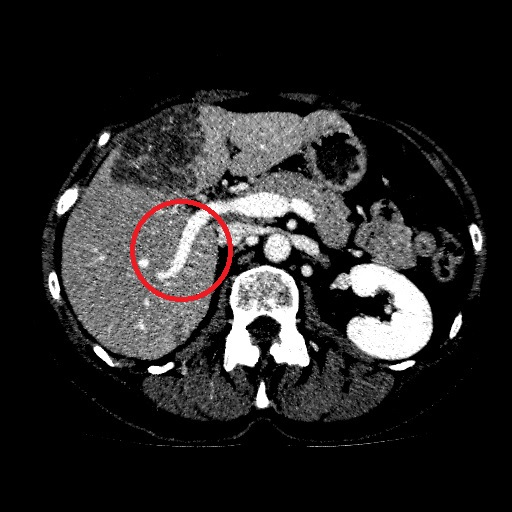
\includegraphics[width=.3\textwidth]{figures/portal_vein}
		\caption{Tĩnh mạch cửa trong cơ quan gan.}
		\label{fig:portal_vein}
	\end{figure}
	Về kích thước của mạch máu, theo tài liệu \cite{covey2004incidence}, tĩnh mạch cửa là mạch máu có đường kính lớn nhất trong cơ quan gan (\autoref{fig:portal_vein}) với độ lớn đường kính trong khoảng 15 -- 18mm. Đối chiếu với kích thước nội suy dữ liệu cho mỗi điểm ảnh 1mm(W)$\times$1mm(H)$\times$1mm(D) sẽ được trình bày trong \autoref{subsec:noi_suy_du_lieu}, đường kính tĩnh mạch cửa sẽ nằm trong khoảng\linebreak 15 -- 18 điểm ảnh. Độ lớn kích thước receptive field của mô hình phải phù hợp với ngưỡng\linebreak giá trị này.
	
	\begin{table}[h!]
		\centering
		\caption{Kích thước receptive field qua mỗi lớp mạng trên nhánh trái kiến trúc U-Net.}
		\label{tab:unet_receptive_field}
		\begin{tabular}{crrr}
			\toprule
			\textbf{Tầng} & \multicolumn{1}{l}{\textbf{Convolution 1}} & \multicolumn{1}{l}{\textbf{Convolution 2}} & \multicolumn{1}{l}{\textbf{Max-pooling}} \\ \midrule
			1 & 3 & 5 & 6 \\[1mm]
			2 & 10 & 14 & 16 \\[1mm]
			3 & 24 & 32 & 36 \\[1mm]
			4 & 52 & 68 & 76 \\[1mm]
			5 & 108 & 140 &  \_\\ \bottomrule
		\end{tabular}
	\end{table}
	Về kích thước receptive field\index{Receptive field}, chúng tôi tiến hành tính toán trên mỗi lớp mạng ở nhánh trái của mô hình U-Net (nhánh phải đối xứng thông qua sử dụng phép copy và concat) và thu được kết quả như \autoref{tab:unet_receptive_field}. Từ số liệu thu được, chúng tôi nhận thấy kích thước receptive field ở tầng 4 và 5 lớn hơn rất nhiều so với kích thước mạch máu đã nêu ở trên, chúng tôi đề xuất độ sâu của mô hình U-Net* là 3 tầng thay vì 5 tầng như trong kiến trúc U-Net. Tính hiệu quả của mô hình trước và sau thay đổi số tầng được chúng tôi trình bày trong \autoref{sec:ket_qua_thi_nghiem}.

	\begin{figure}[h!]
		\hspace*{-1.5mm}\begin{tikzpicture}[scale=.25]
	\definecolor{boxfill}{RGB}{114, 159, 207};
	\definecolor{boxoutline}{RGB}{57, 106, 167};
	\definecolor{arrowcvbnre}{RGB}{0, 0, 128};
	\definecolor{arrowconcat}{RGB}{198, 198, 198};
	\definecolor{arrowmapool}{RGB}{128, 0, 0};
	\definecolor{arrowupconv}{RGB}{0, 123, 0};
	\definecolor{arrowsoftcv}{RGB}{0, 176, 240};
	\definecolor{colornumber}{RGB}{100, 100, 100};
	
	% \drawbox#x#y#width#height#fillcolor
	\def\drawbox#1#2#3#4#5{
		\draw[fill=#5, draw=boxoutline, very thick]  (#1, #2) rectangle (#1 + #3, #2 - #4);
	}

	% \drawarrow#x1#y1#x2#y2#color
	\def\drawarrow#1#2#3#4#5{
		\draw[->, >={Triangle[width=2.5mm, length=2mm]}, line width=1.5mm, #5]  (#1, #2) -- (#3, #4);
	}

	% \drawnodeh#x#y#label
	\def\drawnodeh#1#2#3{
		\node[above] at (#1, #2) {\scriptsize\sffamily\textcolor{colornumber}{#3}};
	}

	% \drawnodev#x#y#label
	\def\drawnodev#1#2#3{
		\node[rotate=90, yshift=1.75mm] at (#1, #2) {\scriptsize\sffamily\textcolor{colornumber}{#3}};
	}

	% model
	\drawbox{0}{0}{.25}{10}{boxfill}\drawnodev{0}{-9}{112\textsuperscript{3}}\drawnodeh{.125}{0}{1}
	\drawarrow{.5}{-5}{1.75}{-5}{arrowcvbnre}
	\drawbox{2}{0}{1}{10}{boxfill}\drawnodev{2}{-9}{112\textsuperscript{3}}\drawnodeh{2.5}{0}{64}
	\drawarrow{3.25}{-5}{4.5}{-5}{arrowcvbnre}
	\drawbox{4.75}{0}{1}{10}{boxfill}\drawnodev{4.75}{-9}{112\textsuperscript{3}}\drawnodeh{5.25}{0}{64}
	
	\drawarrow{5.25}{-10.5}{5.25}{-12.5}{arrowmapool}
	
	\drawbox{4.75}{-13}{1}{5}{boxfill}\drawnodev{4.75}{-18}{56\textsuperscript{3}}
	\drawarrow{6}{-15.5}{7.25}{-15.5}{arrowcvbnre}
	\drawbox{7.5}{-13}{2}{5}{boxfill}\drawnodev{7.5}{-18}{56\textsuperscript{3}}\drawnodeh{8.5}{-13}{128}
	\drawarrow{9.75}{-15.5}{11}{-15.5}{arrowcvbnre}
	\drawbox{11.25}{-13}{2}{5}{boxfill}\drawnodev{11.25}{-18}{56\textsuperscript{3}}\drawnodeh{12.25}{-13}{128}
	
	\drawarrow{12.25}{-18.5}{12.25}{-20.5}{arrowmapool}
	
	\drawbox{11.25}{-21}{2}{2}{boxfill}\drawnodev{11.25}{-24}{28\textsuperscript{3}}
	\drawarrow{13.5}{-22}{14.75}{-22}{arrowcvbnre}
	\drawbox{15}{-21}{4}{2}{boxfill}\drawnodev{15}{-24}{28\textsuperscript{3}}\drawnodeh{17}{-21}{256}
	\drawarrow{19.25}{-22}{20.5}{-22}{arrowcvbnre}
	\drawbox{20.75}{-21}{4}{2}{boxfill}\drawnodev{20.75}{-24}{28\textsuperscript{3}}
	
	\drawarrow{23.75}{-20.5}{23.75}{-18.5}{arrowupconv}
	
	\drawbox{20.75}{-13}{2}{5}{none}\drawnodev{20.75}{-18}{56\textsuperscript{3}}
	\drawbox{22.75}{-13}{2}{5}{boxfill}\drawnodeh{22.75}{-13}{256}
	\drawarrow{25}{-15.5}{26.25}{-15.5}{arrowcvbnre}
	\drawbox{26.5}{-13}{2}{5}{boxfill}\drawnodev{26.5}{-18}{56\textsuperscript{3}}\drawnodeh{27.5}{-13}{128}
	\drawarrow{28.75}{-15.5}{30}{-15.5}{arrowcvbnre}
	\drawbox{30.25}{-13}{2}{5}{boxfill}\drawnodev{30.25}{-18}{56\textsuperscript{3}}
	
	\drawarrow{31.5}{-12.5}{31.5}{-10.5}{arrowupconv}
	
	\drawbox{30.25}{0}{1}{10}{none}\drawnodev{30.25}{-9}{112\textsuperscript{3}}
	\drawbox{31.25}{0}{1}{10}{boxfill}\drawnodeh{31.25}{0}{128}
	\drawarrow{32.5}{-5}{33.75}{-5}{arrowcvbnre}
	\drawbox{34}{0}{1}{10}{boxfill}\drawnodev{34}{-9}{112\textsuperscript{3}}\drawnodeh{34.5}{0}{64}
	\drawarrow{35.25}{-5}{36.5}{-5}{arrowcvbnre}
	\drawbox{36.75}{0}{1}{10}{boxfill}\drawnodev{36.75}{-9}{112\textsuperscript{3}}\drawnodeh{37.25}{0}{64}
	\drawarrow{38}{-5}{39.25}{-5}{arrowsoftcv}
	\drawbox{39.5}{0}{.25}{10}{boxfill}\drawnodev{39.5}{-9}{112\textsuperscript{3}}\drawnodeh{39.625}{0}{2}
	
	\drawarrow{8}{-5}{28}{-5}{arrowconcat}
	\drawarrow{15.5}{-15.5}{18.5}{-15.5}{arrowconcat}
	
	\node[align=right, left] at (0, -3) {\sffamily input\\\sffamily volume\\\sffamily data};
	\node[align=left, right] at (39.75, -5) {\sffamily output\\\sffamily segmentation\\\sffamily map};
	
	% legend
	\drawarrow{35.5}{-14}{36.75}{-14}{arrowcvbnre}
	\node[right] at (37, -14) {\sffamily\textcolor{arrowcvbnre}{conv 3x3x3, (batchnorm), ReLU}};
	\drawarrow{35.5}{-16.5}{36.75}{-16.5}{arrowconcat}
	\node[right] at (37, -16.5) {\sffamily\textcolor{colornumber}{copy and concat}};
	\drawarrow{36.2}{-18.375}{36.2}{-19.625}{arrowmapool}
	\node[right] at (37, -19) {\sffamily\textcolor{arrowmapool}{max-pool 2x2x2}};
	\drawarrow{36.2}{-22.125}{36.2}{-20.875}{arrowupconv}
	\node[right] at (37, -21.5) {\sffamily\textcolor{arrowupconv}{up-conv 2x2x2}};
	\drawarrow{35.5}{-24}{36.75}{-24}{arrowsoftcv}
	\node[right] at (37, -24) {\sffamily\textcolor{arrowsoftcv}{conv 1x1x1}};
\end{tikzpicture}
		\caption{Kiến trúc mô hình U-Net*.}
		\label{fig:model_unet_star}
	\end{figure}
	Và tương tự như DeepVesselNet, chúng tôi đề xuất bổ sung lớp batchnorm trước các lớp ReLU trong kiến trúc này để đánh giá, so sánh. \autoref{fig:model_unet_star} mô tả chi tiết kiến trúc mô hình U-Net* với độ sâu kiến trúc là 3, sử dụng convolution 3D và tuỳ chọn bổ sung các lớp batchnorm.
	
	Bên cạnh các đề xuất đã nêu ở trên, do hiểu được ưu điểm của các mạng như DenseNet và ResNet, chúng tôi đề xuất kết hợp các mô hình này vào các mô hình đang có để tiến hành thí nghiệm và so sánh, đánh giá. Kết quả thí nghiệm được chúng tôi trình bày\linebreak trong \autoref{sec:ket_qua_thi_nghiem}.

\subsection{Hàm lỗi} 
\label{subsec:ham_loi}
	Chúng tôi sử dụng hai hàm lỗi trong huấn luyện hệ thống. Hàm thứ nhất là cross entropy cải tiến như trong \autoref{eqn:crossentropy_fpcorrection}. Hàm lỗi thứ hai chúng tôi đề xuất sử dụng hàm lỗi Dice. Đây là hàm lỗi thường được sử dụng cho các bài toán mất cân bằng lớp.
	
	Hàm lỗi Dice lần đầu tiên được đề xuất bởi Milletari và cộng sự \cite{milletari2016v} dựa trên hệ số Dice. Bằng cách này, chúng ta có thể giải quyết các trường hợp mà sự mất cân bằng giữa foreground\index{Foreground} và background\index{Background} quá lớn. Công thức hàm lỗi Dice được mô tả như sau
	\begin{equation}
		Diceloss = 1 - 2\dfrac{\sum_{i=1}^{N} Y_i * P_i + 1}{\sum_{i=1}^{N} (Y_i + P_i) + 1},
		\label{eqn:diceloss}
	\end{equation}
	trong đó, $N$ là tổng số điểm ảnh, $Y_i$ và $P_i$ là giá trị nhãn thực sự và giá trị dự đoán của điểm ảnh thứ $i$, với $Y_i \in \{0, 1\}$ và $P_i \in [0, 1]$.

\newpage
\section{Tìm đường chính giữa và điểm phân nhánh} 
\label{sec:tim_duong_chinh_giua_va_diem_phan_nhanh}
	Hai nhiệm vụ chúng tôi sẽ thực hiện sau khi xây dựng hệ thống mạch máu đó là tìm đường chính giữa và xác định điểm phân nhánh. Điều này có ý nghĩa rất quan trọng trong việc xác định vị trí tương quan giữa các phân thuỳ gan, giúp công tác giải phẫu có thể tiến hành nhanh chóng và an toàn hơn.
	
	Đối với tìm đường chính giữa của mạch máu, chúng tôi áp dụng phép toán skeleton để trích xuất khung xương đối tượng trong không gian 3D như đã trình bày trong \autoref{subsec:phep_toan_skeleton}.\linebreak Trong luận văn này chúng tôi thực hiện phép toán skeleton thông qua hàm \verb/skeletonize_3d/ trong gói \verb/morphology/ của thư viện \verb/skimage/ trên ngôn ngữ Python..
	
	Đối với xác định điểm phân nhánh, chúng tôi xem xét số lượng điểm ảnh liền kề thuộc khung xương của từng điểm ảnh trong khung xương mạch máu. Một điểm ảnh là điểm phân nhánh khi và chỉ khi số lượng điểm ảnh thuộc khung xương liền kề nó lớn hơn hoặc bằng 3. \autoref{fig:post_processing_branching_point} minh hoạ việc xác định điểm phân nhánh trên khung xương mạch máu. Trong đó, các điểm được tô màu mô tả khung xương mạch máu và điểm màu cam là các điểm phân nhánh trên khung xương đó.
	\begin{figure}[h!]
		\centering
		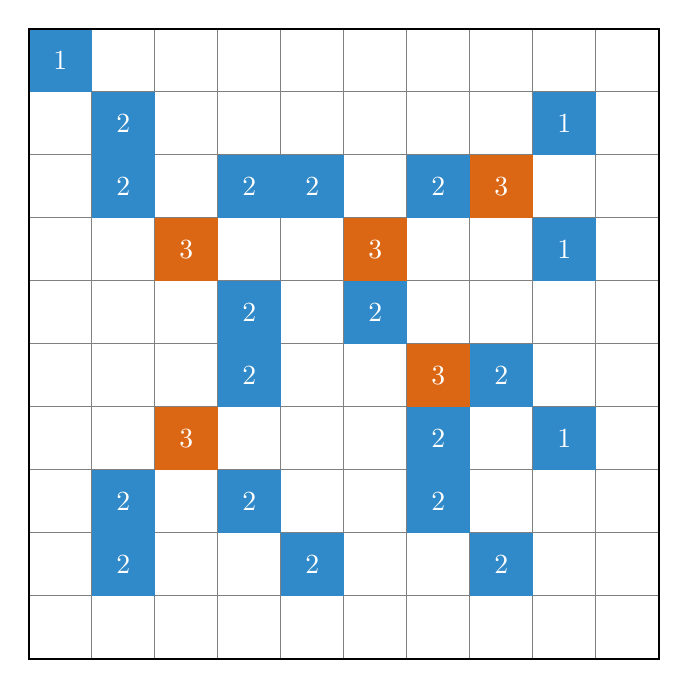
\begin{tikzpicture}[thick, scale=.8]

	\def\colors{{
		"048 137 201", % 1 adjacency points
		"048 137 201", % 2 adjacency points
		"219 103 020"  % 3 adjacency points
	}}

	% index x
	\def\posx{{
		0,
		   1,                   8,
		   1,    3, 4,    6, 7,
		      2,       5,       8,
		         3,    5,
		         3,       6, 7,
		      2,          6,    8,
		   1,    3,       6,
		   1,       4,       7
	}}

	% index y
	\def\posy{{
		9,
		   8,                   8,
		   7,    7, 7,    7, 7,
		      6,       6,       6,
		         5,    5,
		         4,       4, 4,
		      3,          3,    3,
		   2,    2,       2,
		   1,       1,       1
	}}

	% the number of adjacency points
	\def\neighbors{{
		1,
		   2,                   1,
		   2,    2, 2,    2, 3,
		      3,       3,       1,
		         2,    2,
		         2,       3, 2,
		      3,          2,    1,
		   2,    2,       2,
		   2,       2,       2
	}}

	% \drawsquare#x#y#size#label#fillcolor#drawcolor
	\def\drawsquare#1#2#3#4#5#6{
		\filldraw[fill=#5, draw=#6] (#1, #2) rectangle (#1 + #3, #2 + #3) node[pos=.5] {\textcolor{white}{#4}};
	}

	% grid
	\draw[very thin, color=gray] (0, 0) grid (10, 10);

	% pixel
	\foreach \i in {0, ..., 24} {
		\def\neighbor{\neighbors[\i]}
		\pgfmathparse{\colors[\neighbor - 1]};
		\definecolor{color}{RGB}{\pgfmathresult};
		\drawsquare{\posx[\i]}{\posy[\i]}{1}{\pgfmathparse{\neighbor}\pgfmathresult}{color}{none}
	}

	% frame
	\drawsquare{0}{0}{10}{}{none}{black}
\end{tikzpicture}

%%%%%%%%%%%%%%%%%%%%%%%%%%%%%%%%%%%%%%%%%%%%%%%%
% Bellow is old version
%%%%%%%%%%%%%%%%%%%%%%%%%%%%%%%%%%%%%%%%%%%%%%%%

%\begin{tikzpicture}[thick, scale=.8]
%	\def\colors{{
%		"000 000 000", % black
%		"255 255 255", % white
%		"255 255 255", % white
%		"255 000 000"  % red
%	}}
%
%	% \drawsquare#x#y#size#label#color
%	\def\drawsquare#1#2#3#4#5{
%		\filldraw[fill=#5] (#1, #2) rectangle (#1 + #3, #2 + #3) node[pos=.5] {#4};
%	}
%	
%	% vessel
%	\def\neighbors{{
%		1, 0, 0, 0, 0, 0, 0, 0, 0,
%		0, 2, 0, 0, 0, 0, 0, 0, 1,
%		0, 2, 0, 2, 2, 0, 2, 3, 0,
%		0, 0, 3, 0, 0, 3, 0, 0, 1,
%		0, 0, 0, 2, 0, 2, 0, 0, 0,
%		0, 0, 0, 2, 0, 0, 3, 2, 0,
%		0, 0, 3, 0, 0, 0, 2, 0, 1,
%		0, 2, 0, 2, 0, 0, 2, 0, 0,
%		0, 2, 0, 0, 2, 0, 0, 2, 0
%	}}
%	
%	% board
%	\drawsquare{0}{0}{10}{0}{black}
%	
%	% pixel
%	\foreach \y in {0, ..., 8} {
%		\foreach \x in {0, ..., 8} {
%			\def\neighbor{\neighbors[9 * \y + \x]}
%			\pgfmathparse{\colors[\neighbor]};
%			\definecolor{color}{RGB}{\pgfmathresult};
%			\drawsquare{\x}{9 - \y}{1}{\pgfmathparse{\neighbor}\pgfmathresult}{color}
%		}
%	}
%\end{tikzpicture}
		\caption[Phương pháp xác định điểm phân nhánh mạch máu.]{Phương pháp xác định điểm phân nhánh mạch máu. Các điểm được tô màu mô phỏng khung xương mạch máu. Con số trên mỗi điểm là số lượng điểm ảnh kế cận thuộc khung xương của điểm đó. Các điểm tô màu cam là các điểm phân nhánh.}
		\label{fig:post_processing_branching_point}
	\end{figure}

